\documentclass[oneside,a4paper,14pt]{extarticle}
\usepackage[a4paper,letterpaper,top=20mm,bottom=20mm,left=20mm,right=10mm]{geometry}
\usepackage[russian]{babel}
\usepackage{textcomp}
\usepackage{indentfirst}
\usepackage{graphicx}
\usepackage{mwe}
\usepackage{wrapfig}
\usepackage{caption}
\usepackage{amsmath}
\usepackage{amsfonts}
\usepackage{amsthm}
\usepackage{amssymb}
\usepackage[all]{xy}
\usepackage[breaklinks]{hyperref}
\usepackage{titlesec}
\usepackage{xcolor}
\usepackage{nicematrix}
\usepackage{multirow}
\usepackage{tikz}

\titleformat{\section} % Настройка формата заголовков секций
{\normalsize\bfseries} % Устанавливает размер шрифта на нормальный и делает его жирным
{\thesection} % Указывает, что номер секции будет отображаться перед заголовком
{1em} % Устанавливает расстояние между номером секции и заголовком в 1em
{} % Дополнительные параметры.

\titleformat{\subsection} % Настройка формата заголовков подсекций
{\normalsize\bfseries} % Устанавливает размер шрифта на нормальный и делает его жирным
{\thesubsection} % Указывает, что номер подсекции будет отображаться перед заголовком
{1em} % Устанавливает расстояние между номером подсекции и заголовком в 1em
{} % Дополнительные параметры.

\titleformat{\subsubsection} % Настройка формата заголовков подподсекций
{\normalsize\bfseries} % Устанавливает размер шрифта на нормальный и делает его жирным
{\thesubsection} % Указывает, что номер подподсекции будет отображаться перед заголовком
{1em} % Устанавливает расстояние между номером подподсекции и заголовком в 1em
{} % Дополнительные параметры.

\renewcommand\baselinestretch{1.45}\normalsize %межстр интервал
\setlength{\parindent}{1.25cm} %длина отступа нового абзаца

\begin{document}
\newpage
\thispagestyle{empty}
\begin{center}
	МИНИСТЕРСТВО НАУКИ И ВЫСШЕГО ОБРАЗОВАНИЯ\\
	РОССИЙСКОЙ ФЕДЕРАЦИИ
	ФЕДЕРАЛЬНОЕ ГОСУДАРСТВЕННОЕ БЮДЖЕТНОЕ\\
	ОБРАЗОВАТЕЛЬНОЕ
	УЧРЕЖДЕНИЕ ВЫСШЕГО ОБРАЗОВАНИЯ\\
	«ВЯТСКИЙ ГОСУДАРСТВЕННЫЙ УНИВЕРСИТЕТ»\\
	Институт математики и информационных систем\\
	Факультет автоматики и вычислительной техники\\
	Кафедра электронных вычислительных машин
\end{center}
\vspace{20mm}

\begin{center}
	Отчёт по лабораторной работе №8\\
	по дисциплине\\
	<<Информатика>>\\
	<<Разработка последовательных схем (счётчиков).>>\\
\end{center}
\vspace{40mm}
\noindent
\begin{tabular}{ll}
	Разработал студент гр. ИВТб-1301-05-00 & \rule[-1mm]{30mm}{0.10mm}\,/Черкасов А. А./ \\
	                                       & \hspace{8mm}\footnotesize(подпись)          \\

	Проверил доцент кафедры ЭВМ            & \rule[-1mm]{30mm}{0.10mm}\,/Коржавина А.С./ \\
	                                       & \hspace{8mm}\footnotesize(подпись)          \\
\end{tabular}

\vfill
\begin{center}
	Киров\\
	2024
\end{center}

\newpage\thispagestyle{plain}
\section*{Цель работы}
Цель работы: Закрепить на практике знания об элементах памяти и последовательных устройствах и получить навыки их реализации.\\
\section*{Задания}
\begin{enumerate}
	\item
	      Построить схемы прямого (на +1) и обратного (на -1) 4-разрядных
	      двоичных счетчиков на счетных (T) триггерах.
	\item
	      Построить схему прямого счетчика по модулю 10, то есть считающего
	      в прямом направлении от 0 до 9 на счетных (T) триггерах.
	\item
	      Построить схему прямого счетчика по произвольному модулю N, то
	      есть считающего в прямом направлении от 0 до N-1 на счетных (T) триггерах.
	      Построить схему счетчика в Logisim, проверить его работоспособность.
	\item
	      Построить схему прямого счетчика по произвольному модулю N, то
	      есть считающего в прямом направлении от 0 до N-1 на D триггерах.
	      Построить схему счетчика в Logisim, проверить его работоспособность.
	\item 
		  Построить схему прямого счетчика на +3. Счетчик увеличивает значение на
		  +3, то есть счет идет 0 3 6 9 12 15 0 и т.д. на T триггерах. Построить схему
		  счетчика в Logisim, проверить его работоспособность.
	\item 
		  Построить схему прямого счетчика на +5. Счетчик увеличивает значение на
		  +5, то есть счет идет 0 5 10 15 20 25 30 0 и т.д. на T триггерах. Построить
		  схему счетчика в Logisim, проверить его работоспособность.
\end{enumerate}
\newpage

\section*{Решение}

\section*{Задание 1}
Схемы прямого и обратного 4-разрядных двоичных счетчиков на счетных (T) триггерах представлены на Рисунках 1.1, 1.2.\\

\begin{figure}[h!]
	\centering
	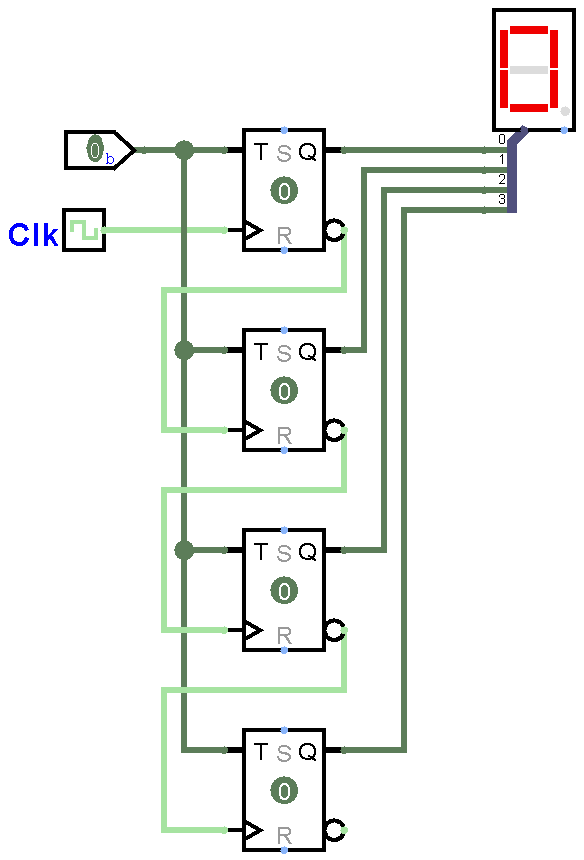
\includegraphics[height=0.7\textheight]{pics/1_1.png}
	\caption*{Рисунок 1.1 - Схема прямого счетчика.}
\end{figure}

\begin{figure}[h!]
	\centering
	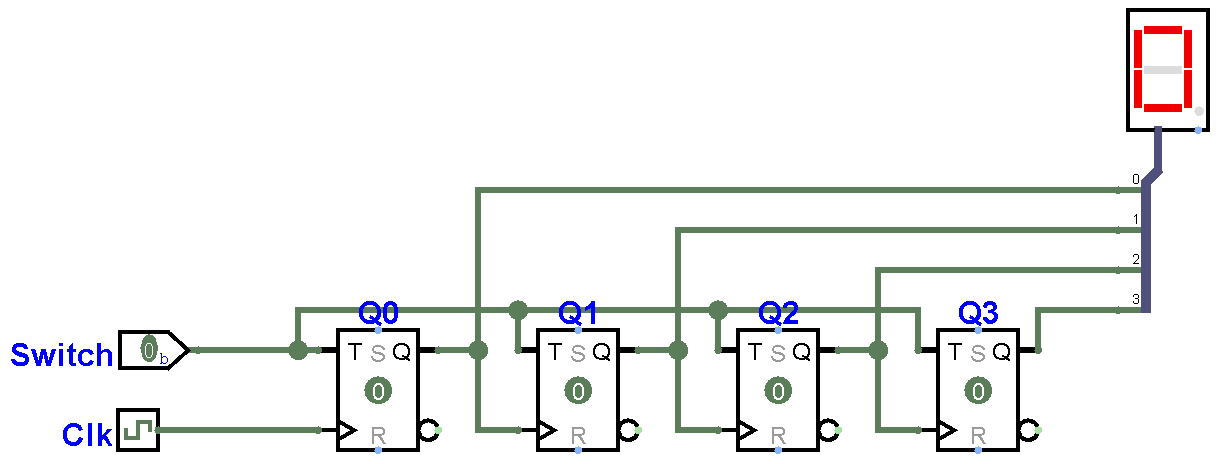
\includegraphics[width=0.75\textwidth]{pics/1_2.png}
	\caption*{Рисунок 1.2 - Схема обратного счетчика.}
\end{figure}

\newpage

\section*{Задание 2}
Схема прямого счетчика по модулю 10 представлена на Рисунке 2.\\

\begin{figure}[h!]
	\centering
	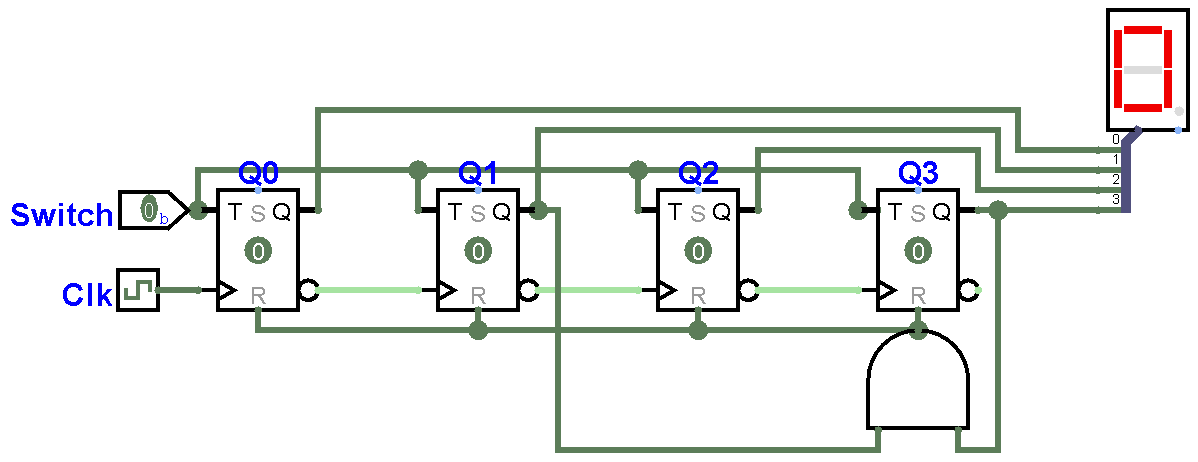
\includegraphics[width=0.75\textwidth]{pics/2.png}
	\caption*{Рисунок 2 - Схема прямого счетчика по модулю 10.}
\end{figure}
\newpage

\section*{Задание 3}
Схема прямого счетчика по произвольному модулю N на (T) триггерах представлена на Рисунке 3.\\

\begin{figure}[h!]
	\centering
	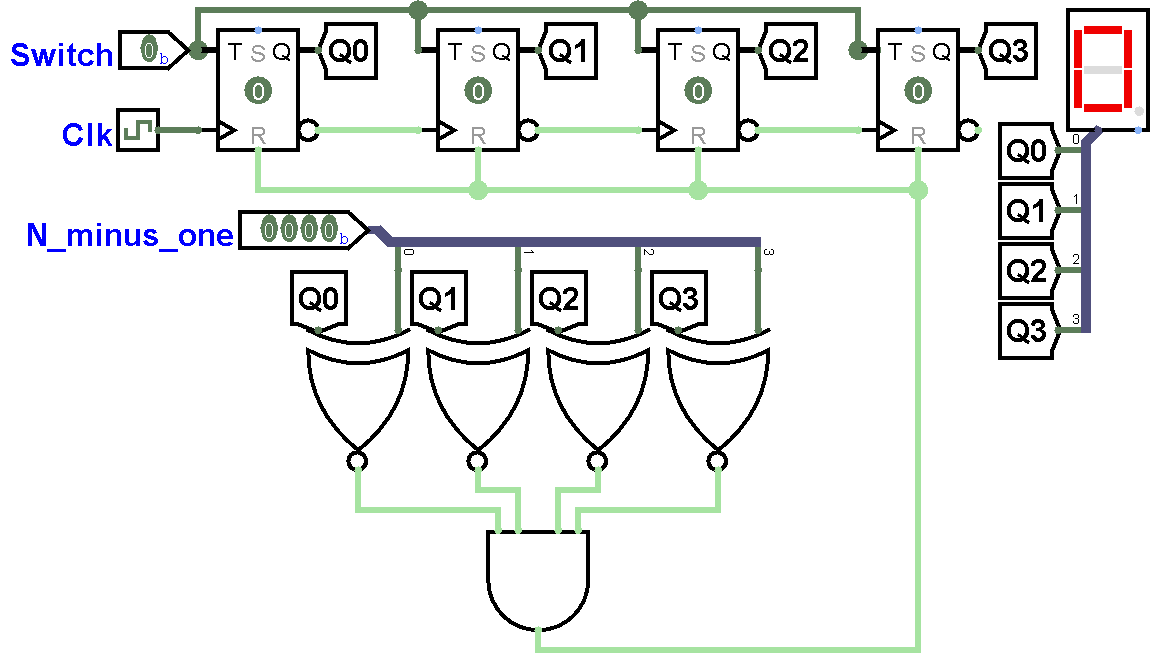
\includegraphics[width=0.8\textwidth]{pics/3.png}
	\caption*{Рисунок 3 - Схема прямого счетчика по произвольному модулю N на (T) триггерах.}
\end{figure}
\newpage

\section*{Задание 4}

Схема прямого счетчика по произвольному модулю N на (D) триггерах представлена на Рисунке 4.\\

\begin{figure}[h!]
	\centering
	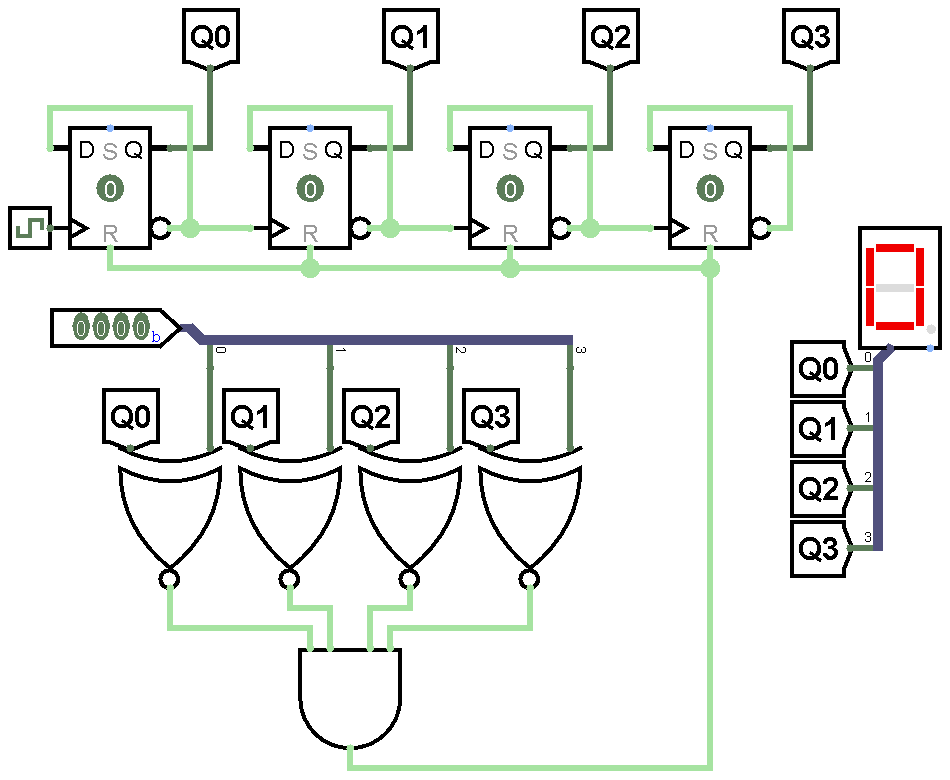
\includegraphics[width=0.95\textwidth]{pics/4.png}
	\caption*{Рисунок 4 - Схема прямого счетчика по произвольному модулю N на (D) триггерах.}
\end{figure}
\newpage

\section*{Задания 5, 6}

Схемы представлены на Рисунках 5.1, 5.2, 5.3, 5.4.\\
\begin{figure}[h!]
	\centering
	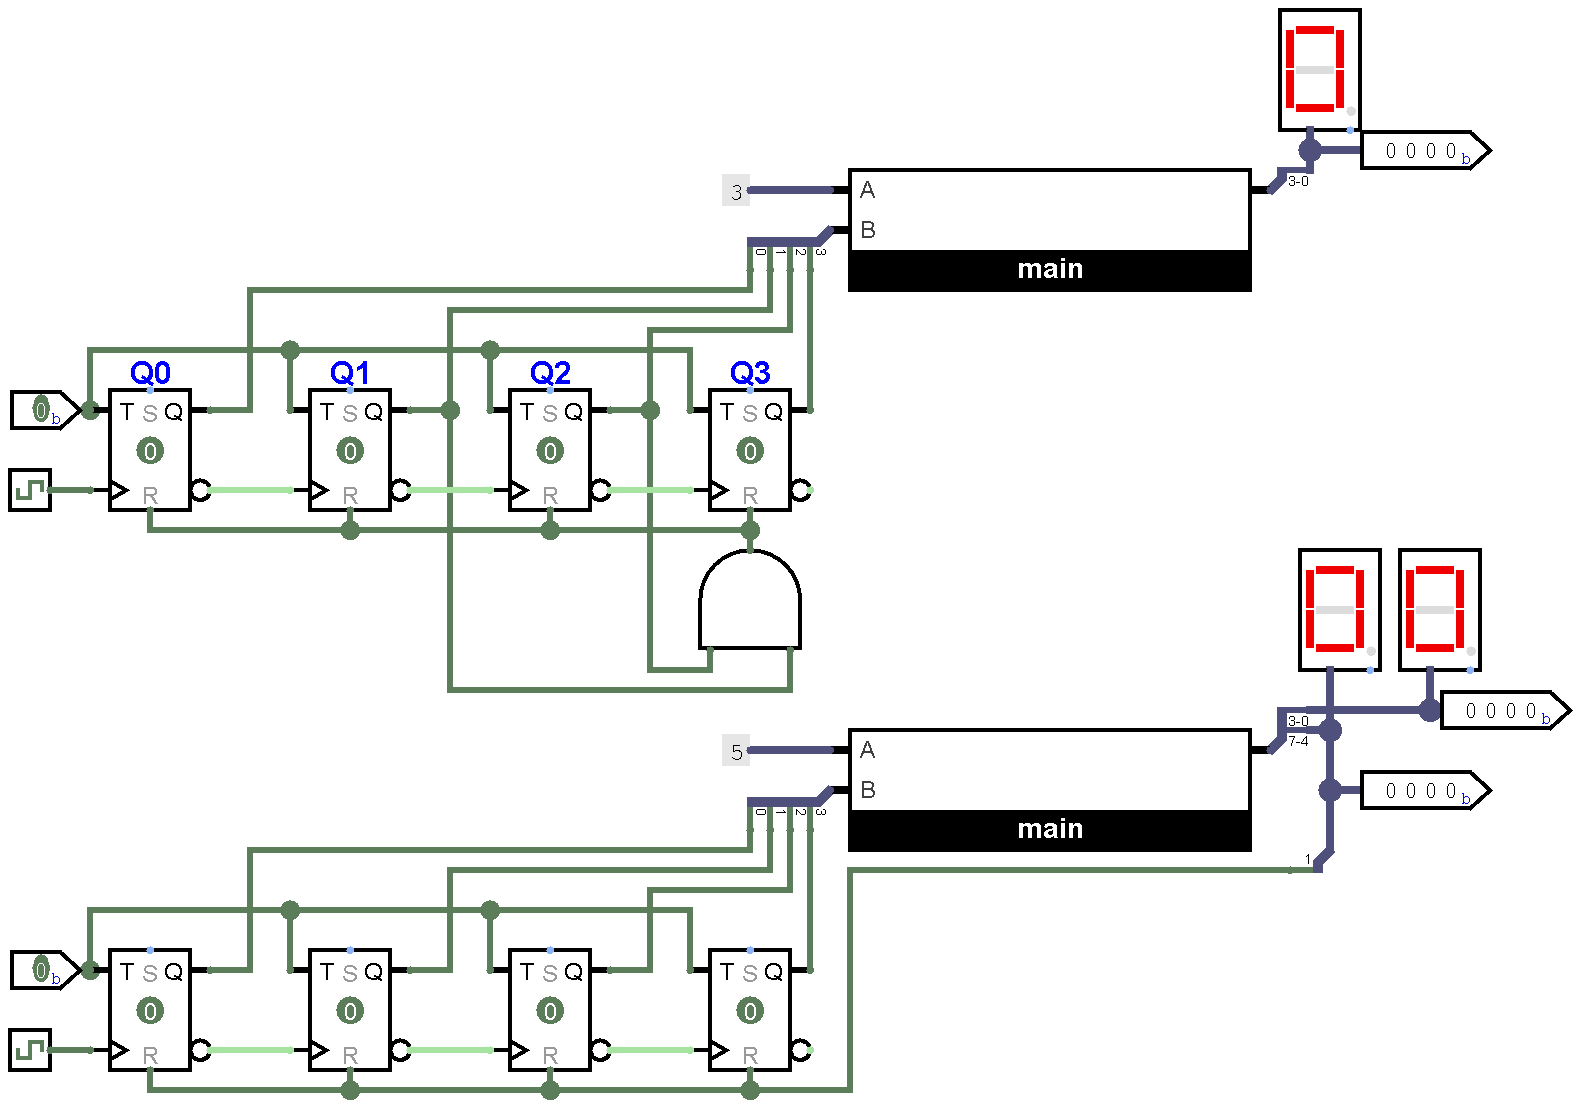
\includegraphics[width=0.95\textwidth]{pics/5.png}
	\caption*{Рисунок 5 - Схемы прямого счетчика на +3 и +5.}
\end{figure}

\begin{figure}[h!]
	\centering
	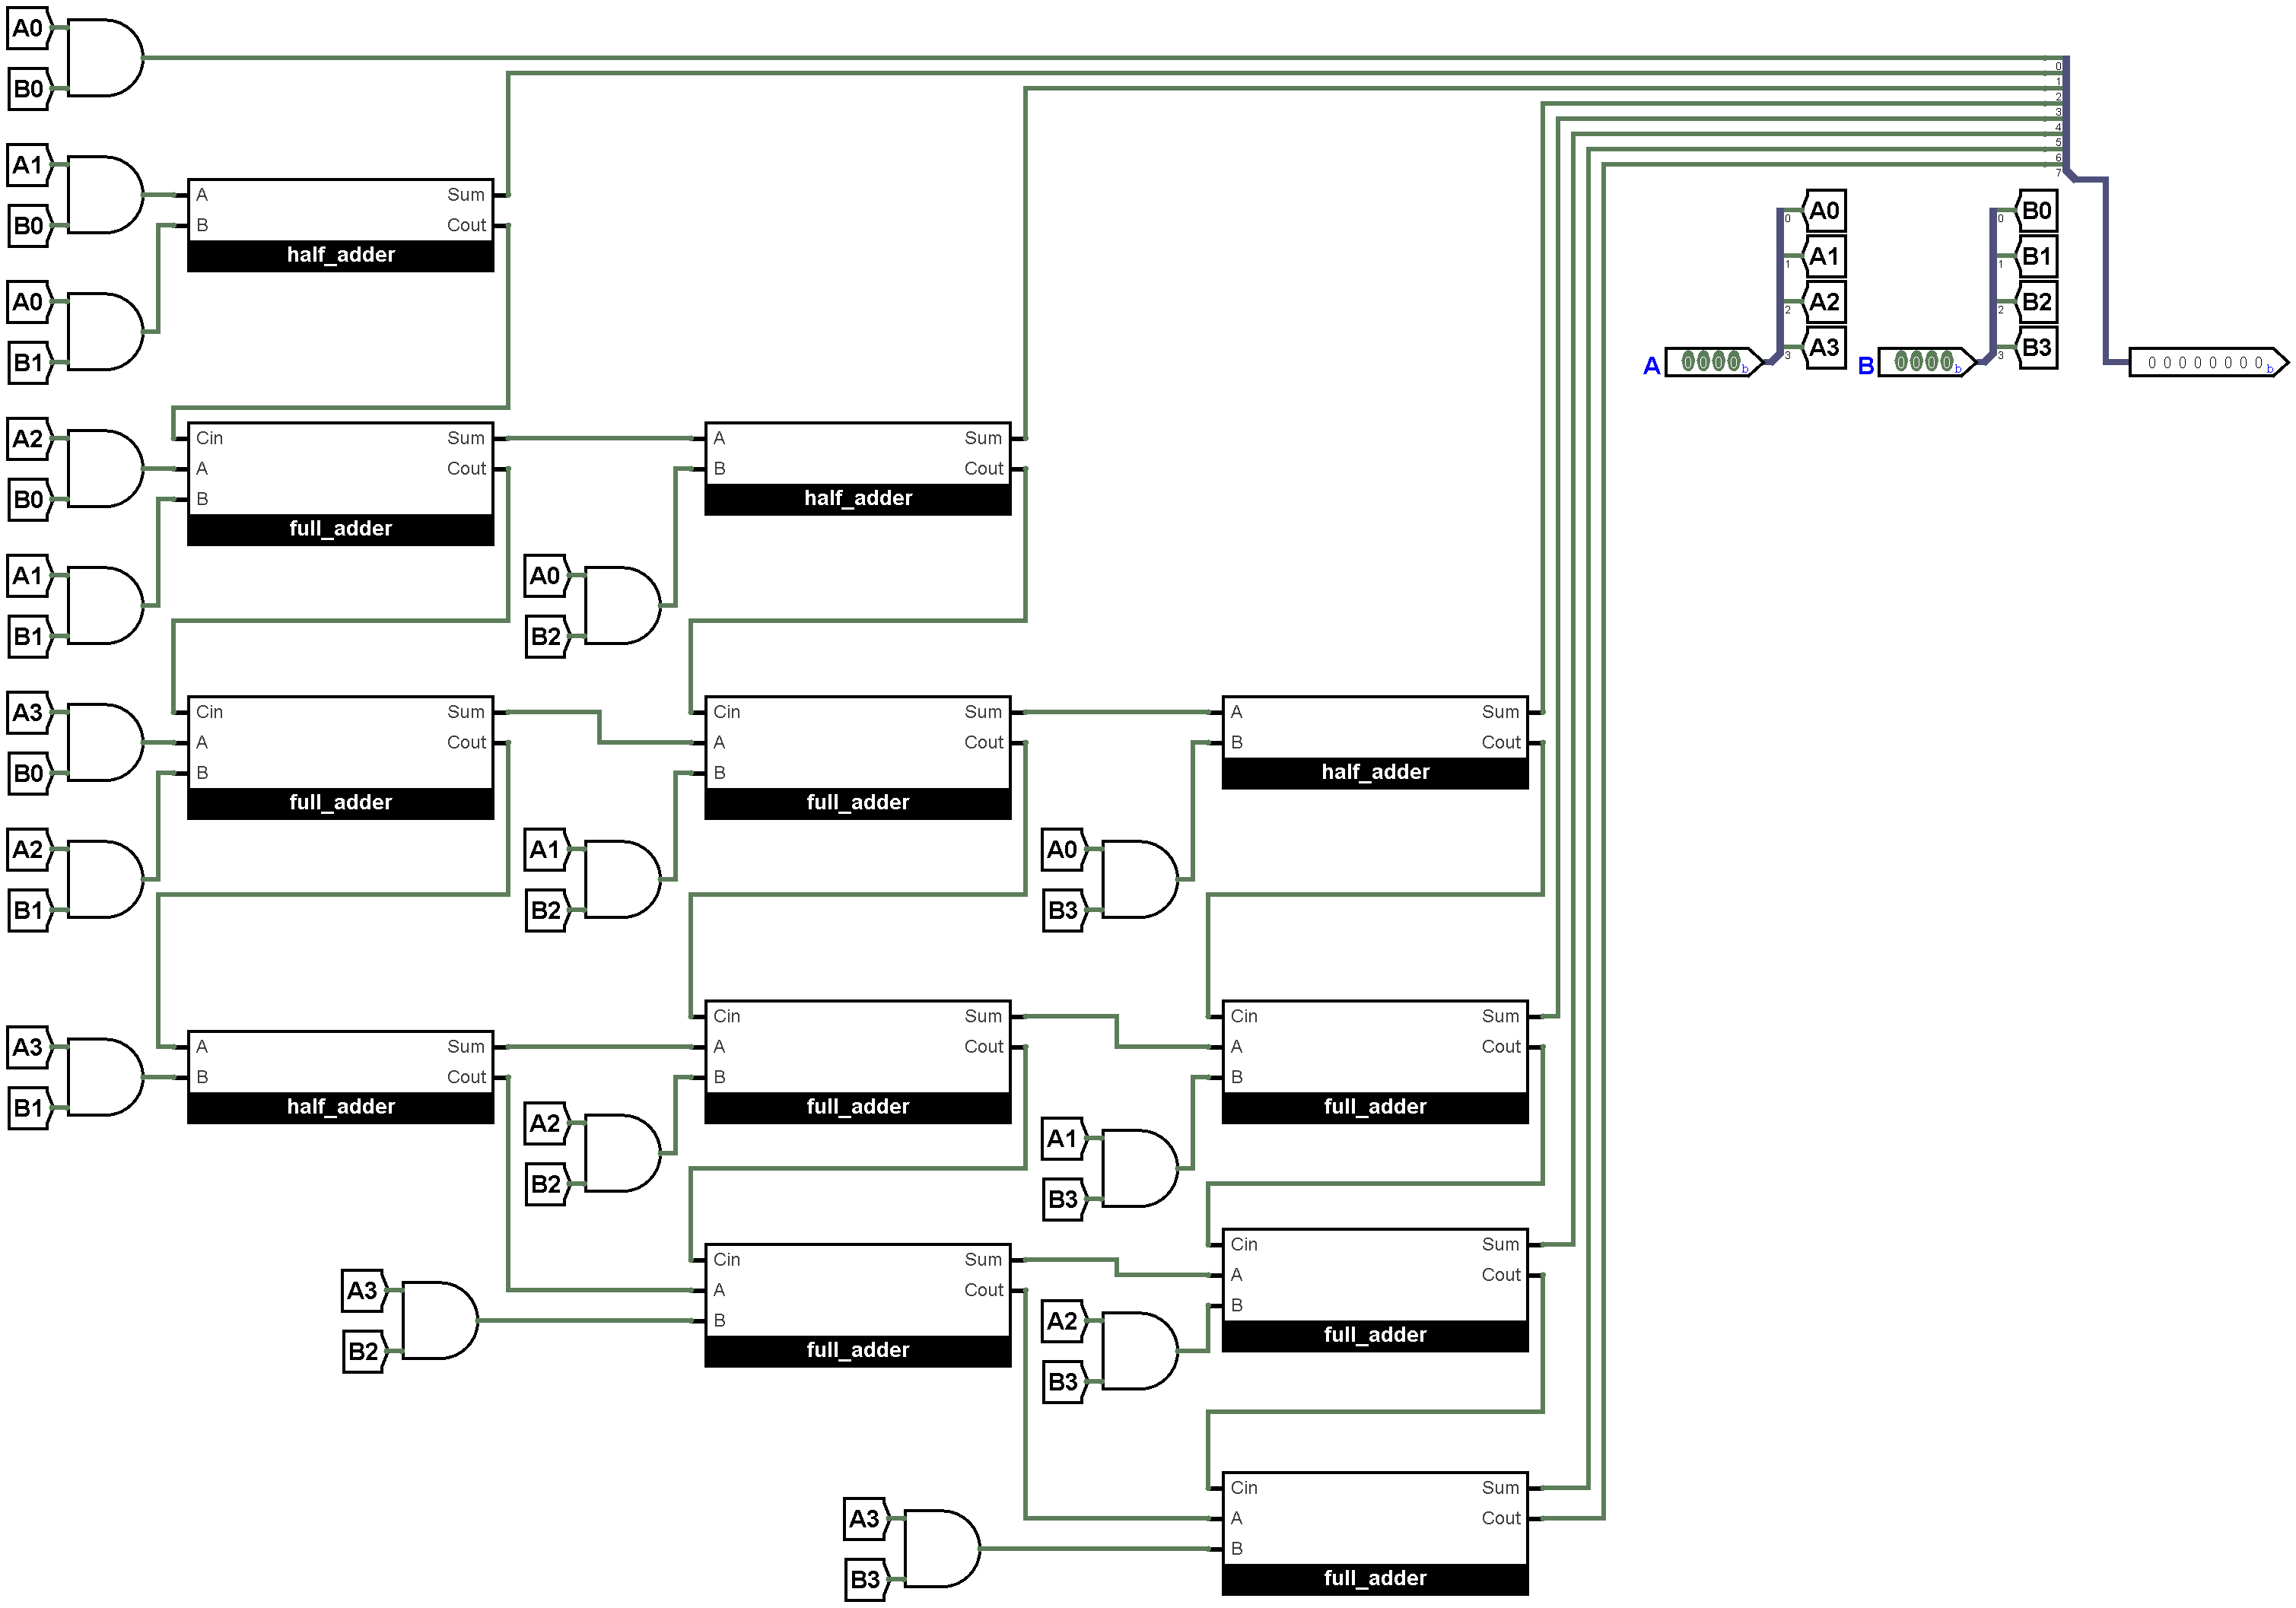
\includegraphics[width=0.95\textwidth]{pics/5_2.png}
	\caption*{Рисунок 5.2 - Схема 4-разрядного умножителя (main).}
\end{figure}

%\begin{figure}[h!]
%	\centering
%	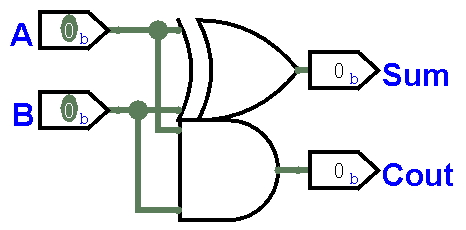
\includegraphics[width=0.5\textwidth]{pics/5_ha.png}
%	\caption*{Рисунок 5.3 - Схема полусумматора.}
%\end{figure}
%
%\begin{figure}[h!]
%	\centering
%	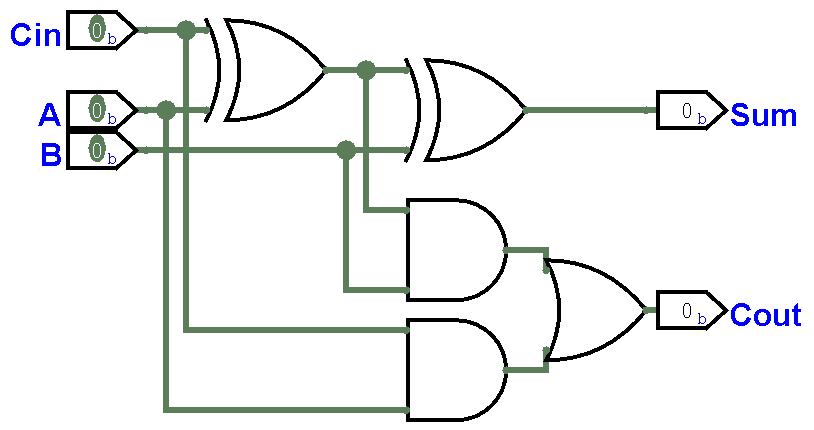
\includegraphics[width=0.5\textwidth]{pics/5_fa.png}
%	\caption*{Рисунок 5.4 - Схема полного сумматора.}
%\end{figure}

\newpage
\section*{Вывод}
В ходе лабораторной работы были закреплены знания об элементах памяти и последовательных устройствах.\\

\end{document}